Die verwendeten Streifenmuster haben entlang ihrer Ausbreitungsrichtung den Grauwerteverlauf einer Rechteckschwingung.

\noindent
Die periodische Einheitsrechteckschwingung $s_f(t)$ sei definiert durch (vgl. \cite{squareWave}):
%
\begin{equation} \label{eq:einheitsrechteckschwingung}
	s_f(t) := \sign \left( \sin \left(2 \pi f t \right) \right)
\end{equation}
%
$\sign(x)$ bezeichnet hierbei die Vorzeichenfunktion mit:
%
\begin{equation*}
	\sign(x) := 
		\begin{cases}
	      -1 & \text{für $x < 0$}\\
	      0 & \text{für $x = 0$}\\
	      1 & \text{für $x > 0$}
	    \end{cases} 
\end{equation*}
%
Die Periodendauer $T$ der Einheitsrechteckschwingung $s_f(t)$ steht über den Kehrwert im Zusammenhang mit der Frequenz $f$:
\begin{equation*}
	T = \dfrac{1}{f}
\end{equation*}
Für $f = \tfrac{1}{3}$ und $f = \tfrac{1}{4}$ sieht das Schaubild der Funktion aus wie in Abbildung \ref{tikz:abbRechteckschwingung}:
% Abbildung: Rechteckschwingung
{
	\begin{figure}[H]
		\centering
		\begin{adjustbox}{width=\textwidth}
	\begin{tikzpicture}
	
		% Koordinatensystem 1
		\draw[thick,-stealth,black] (-8,0)--(8,0) node[below] {$t$};
		\draw[thick,-stealth,black] (0,-2.125)--(0,2.125) node[left] {$s_{\tfrac{1}{3}}(t)$};
		
		% Funktion 1
		\draw[name path = func1, blue, thick, domain=-8:8, samples=600] plot (\x,{1.5*(sign(sin(2*pi*(1/3)*\x r))});

		% Achsenbeschriftungen 1
		\draw[thick,black] (0,-1.5) -- (-0.1,-1.5) node[anchor=east,fill=white] {$-1$};
		\draw[thick,black] (0,1.5) -- (-0.1,1.5) node[anchor=east,fill=white] {$1$};
		\draw[thick,black] (-7,0) -- (-7,-0.1) node[anchor=north,fill=white] {$-7$};
		\draw[thick,black] (-6,0) -- (-6,-0.1) node[anchor=north,fill=white] {$-6$};
		\draw[thick,black] (-5,0) -- (-5,-0.1) node[anchor=north,fill=white] {$-5$};
		\draw[thick,black] (-4,0) -- (-4,-0.1) node[anchor=north,fill=white] {$-4$};
		\draw[thick,black] (-3,0) -- (-3,-0.1) node[anchor=north,fill=white] {$-3$};
		\draw[thick,black] (-2,0) -- (-2,-0.1) node[anchor=north,fill=white] {$-2$};
		\draw[thick,black] (-1,0) -- (-1,-0.1) node[anchor=north,fill=white] {$-1$};
		\draw[thick,black] (1,0) -- (1,-0.1) node[anchor=north,fill=white] {$1$};
		\draw[thick,black] (2,0) -- (2,-0.1) node[anchor=north,fill=white] {$2$};
		\draw[thick,black] (3,0) -- (3,-0.1) node[anchor=north,fill=white] {$3$};
		\draw[thick,black] (4,0) -- (4,-0.1) node[anchor=north,fill=white] {$4$};
		\draw[thick,black] (5,0) -- (5,-0.1) node[anchor=north,fill=white] {$5$};
		\draw[thick,black] (6,0) -- (6,-0.1) node[anchor=north,fill=white] {$6$};
		\draw[thick,black] (7,0) -- (7,-0.1) node[anchor=north,fill=white] {$7$};
		
		% Beschriftung für f
		\draw[blue,thick] node[anchor=west] at (-8,2.125) {$f = \tfrac{1}{3}$:};
		
		
		% Koordinatensystem 2
		\draw[thick,-stealth,black] (-8,-5)--(8,-5) node[below] {$t$};
		\draw[thick,-stealth,black] (0,-7.125)--(0,-2.875) node[left] {$s_{\tfrac{1}{4}}(t)$};
				
		% Funktion 2
		\draw[name path = func2, Green, thick, domain=-8:8, samples=600] plot (\x,{(1.5*(sign(sin(2*pi*(1/4)*\x r)))-5});
				
		% Achsenbeschriftungen 2
		\draw[thick,black] (0,-6.5) -- (-0.1,-6.5) node[anchor=east,fill=white] {$-1$};
		\draw[thick,black] (0,-3.5) -- (-0.1,-3.5) node[anchor=east,fill=white] {$1$};
		\draw[thick,black] (-7,-5) -- (-7,-5.1) node[anchor=north,fill=white] {$-7$};
		\draw[thick,black] (-6,-5) -- (-6,-5.1) node[anchor=north,fill=white] {$-6$};
		\draw[thick,black] (-5,-5) -- (-5,-5.1) node[anchor=north,fill=white] {$-5$};
		\draw[thick,black] (-4,-5) -- (-4,-5.1) node[anchor=north,fill=white] {$-4$};
		\draw[thick,black] (-3,-5) -- (-3,-5.1) node[anchor=north,fill=white] {$-3$};
		\draw[thick,black] (-2,-5) -- (-2,-5.1) node[anchor=north,fill=white] {$-2$};
		\draw[thick,black] (-1,-5) -- (-1,-5.1) node[anchor=north,fill=white] {$-1$};
		\draw[thick,black] (1,-5) -- (1,-5.1) node[anchor=north,fill=white] {$1$};
		\draw[thick,black] (2,-5) -- (2,-5.1) node[anchor=north,fill=white] {$2$};
		\draw[thick,black] (3,-5) -- (3,-5.1) node[anchor=north,fill=white] {$3$};
		\draw[thick,black] (4,-5) -- (4,-5.1) node[anchor=north,fill=white] {$4$};
		\draw[thick,black] (5,-5) -- (5,-5.1) node[anchor=north,fill=white] {$5$};
		\draw[thick,black] (6,-5) -- (6,-5.1) node[anchor=north,fill=white] {$6$};
		\draw[thick,black] (7,-5) -- (7,-5.1) node[anchor=north,fill=white] {$7$};
		
		% Beschriftung für f
		\draw[Green,thick] node[anchor=west] at (-8,-2.875) {$f = \tfrac{1}{4}$:};
		
	\end{tikzpicture}
\end{adjustbox}
\caption[Rechteckschwingung bzw. \textit{engl.: square wave}]{Einheits-Rechteckschwingung (\textit{engl.: square wave}) für $f = \tfrac{1}{3}$ (in blau) und $f = \tfrac{1}{4}$ (in grün).}
		\label{tikz:abbRechteckschwingung}
	\end{figure}
}

\noindent
Mithilfe der Einheitsrechteckschwingung aus Gleichung \ref{eq:einheitsrechteckschwingung} lässt sich ein Streifenmuster mit Ausbreitungsrichtung in $x$ ausdrücken durch:
\begin{equation} \label{eq:rstreifenmuster}
	\begin{gathered}
		m_k(x,y) = A_m 
		\left(
			1 + s_f \left(x - \dfrac{1}{2\pi f} \psi_k \right)
		\right),\\
		f = \dfrac{N_p}{\acrshortmath{lwidth}},
		\quad
		\psi_k = (k - 1)\dfrac{2\pi}{N_{shift}},
		\quad
		k \in \lbrace 1,\ldots,N_{shift}\rbrace 
	\end{gathered}
\end{equation}
%
Das Streifenmuster aus Gleichung \ref{eq:rstreifenmuster} ist durch die Periodizität der Einheitsrechteckschwingung auch periodisch zur Ausbreitungsrichtung.
$A_m$ bezeichnet die Amplitude, $f$ die Frequenz, $N_p$ die Anzahl der Perioden über die Monitorbreite \acrshort{lwidth}, $N_{shift}$ die Anzahl der Phasenverschiebungen und $\psi_k$ die Phasenverschiebung des $k$-ten Musters.
Analog zu Gleichung \ref{eq:rstreifenmuster} lassen sich auch Streifenmuster mit Ausbreitungsrichtung in $y$ über die Monitorhöhe \acrshort{lheight} beschreiben.
Das Bild eines vertikalen Streifenmusters, d. h. mit Ausbreitungsrichtung in $x$, nach Gleichung \ref{eq:rstreifenmuster} wird in Abbildung \ref{tikz:abbRechteckStreifenmuster} dargestellt.

% Abbildung: Rechteck Streifenmuster
{
	\begin{figure}[H]
		\centering
		\begin{adjustbox}{width=\textwidth}
	\begin{tikzpicture}[every node/.style={inner sep=0,outer sep=0}]
	
		\node [anchor=north east] (img1) at (-0.03\textwidth,0) {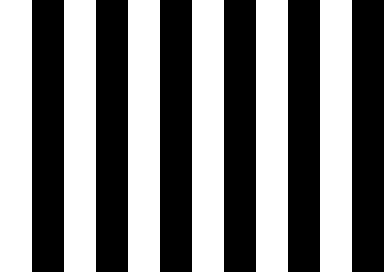
\includegraphics[frame,width=.47\textwidth]{03_sichtpruefungDurchLichtstreuung/einsatzVonMehrerenStreifenmustern/figures/rechteckStreifenmuster}};
		\node [below=0.2cm of img1] {Muster $m_1$ mit $\psi_1 = 0$};
		\node [anchor=north west] (img2) at (0.03\textwidth,0) {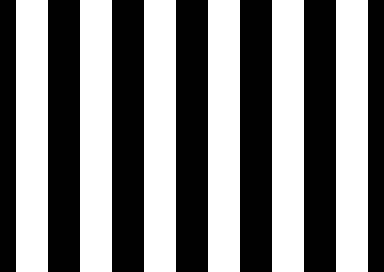
\includegraphics[frame,width=.47\textwidth]{03_sichtpruefungDurchLichtstreuung/einsatzVonMehrerenStreifenmustern/figures/rechteckStreifenmuster_shifted}};
		\node [below=0.2cm of img2] {Muster $m_2$ mit $\psi_2 = \tfrac{\pi}{2}$};
		
	\end{tikzpicture}
\end{adjustbox}
\caption[Rechteckförmiges Streifenmuster]{Streifenmuster nach Gleichung \ref{eq:rstreifenmuster}, mit $A_m = 127.5$, $N_p = 6$, $N_{shift} = 4$ und $\acrshortmath{lwidth} = 384$. Die Breite der Streifen betragen jeweils 32 Pixel.}
		\label{tikz:abbRechteckStreifenmuster}
	\end{figure}
}
%
\noindent
Die verschiedenen Streifenmuster $m_k$ können nach Gleichung \ref{eq:rstreifenmuster} als zueinander phasenverschoben bezeichnet werden.
Die Phasenverschiebung $\psi_k$ wird durch einen Phasenwinkel im Bogenmaß angegeben.
Eine Phasenverschiebung von $ \pi $ bedeutet dementsprechend eine Phasenverschiebung um eine halbe Periode des Musters.
Anschaulich stellt man fest, dass für gleich breite helle und dunkle Streifen diese ihre Positionen tauschen.
Dies kann man sich zunutze machen, denn das bedeutet, dass die Schnittmenge der dunklen Streifen in den beiden Streifenmustern am kleinsten ist.
Da bestimmte Fehlstellen entweder in den dunklen oder in den weißen Streifen deutlich zu erkennen sind, ergänzen sich die beiden Streifenmuster durch die sichtbaren Fehlstellen.
Verknüpft man die Kamerabilder von solchen Mustern, dann kann man damit die meiste Information aus zwei Bildern extrahieren.
Durch zusätzliche Bildaufnahmen mit verschobenen Streifenmustern kann man detailliertere Oberflächeninformationen von dem Prüfobjekt gewinnen.

\begin{figure}[H]
	\centering
	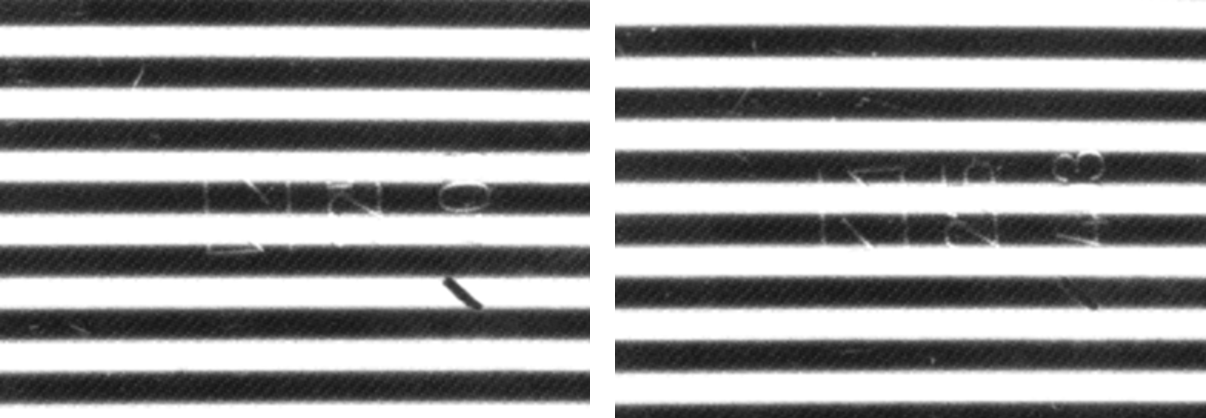
\includegraphics[width=\textwidth]{03_sichtpruefungDurchLichtstreuung/einsatzVonMehrerenStreifenmustern/figures/imageToLink}
	\caption[Zu verknüpfende Bilder]{Kameraaufnahme eines Prüfobjekts unter Projektion von Streifenmustern mit einer Phasenverschiebung von $ \pi $ zueinander.}
	\label{img:imageToLink}
\end{figure}

\noindent
Wie man erkennt, sind die Streifen der beiden Bilder genau zueinander versetzt.
Die Auffälligkeiten in den Bildern wie z. B. Eingravierungen sind oft entweder im dunklen oder im hellen Streifen zu erkennen.
Durch den Unterschied zum Streifenhintergrund erfasst man gewisse Oberflächeninformation des Prüfobjekts.
Das heißt, dass die beiden Bilder sich durch den Versatz in ihrer Oberflächeninformation ergänzen.
Zur Verknüpfung der Information in einem Gesamtbild überlegt man sich, wie bestimmte Defekte in den beiden Bildern aussehen.
Die Defekt- und Fehlstellen werden in zwei Fälle unterteilt (siehe Abbildung \ref{img:imageToLinkWithMarkings}).

\begin{figure}[H]
	\centering
	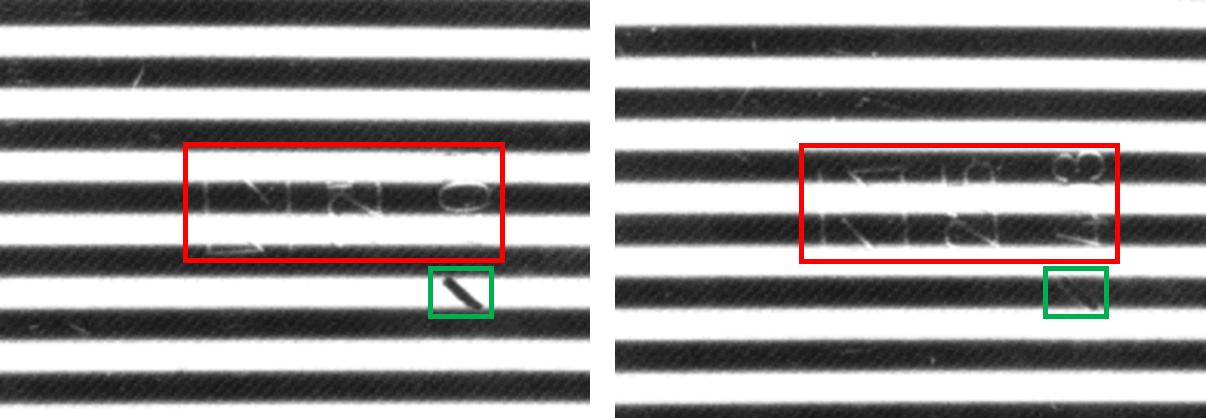
\includegraphics[width=\textwidth]{03_sichtpruefungDurchLichtstreuung/einsatzVonMehrerenStreifenmustern/figures/imageToLinkWithMarkings}
	\caption[Markierte Fehlstellen]{Kameraaufnahme eines Prüfobjekts mit Fehlstellen und deren Kennzeichnung. Im linken Teilbild Aufnahme des Musters $m_1$. Im rechten Teilbild Aufnahme des Musters $m_2$.}
	\label{img:imageToLinkWithMarkings}
\end{figure}

\noindent
\textbf{Fall 1: z. B. Kratzer (siehe rote Rechtecke in Abbildung \ref{img:imageToLinkWithMarkings})}
\nopagebreak
\par\medskip\noindent
\begin{tabular}{@{} p{0.438888889\textwidth} c p{0.438888889\textwidth} @{}}
	Aufnahme von Muster $m_1$ &  & Aufnahme von Muster $m_2$ \\ 
	Helle Fragmente in dunklen Streifen & $ \longleftrightarrow $ & Helle Fragmente in hellen Streifen \\ 
\end{tabular}

\p
\textbf{Fall 2: z. B. Partikel (siehe grüne Rechtecke in Abbildung \ref{img:imageToLinkWithMarkings})}
\nopagebreak
\par\medskip\noindent
\begin{tabular}{@{} p{0.438888889\textwidth} c p{0.438888889\textwidth} @{}}
	Aufnahme von Muster $m_1$ &  & Aufnahme von Muster $m_2$ \\ 
	Dunkle Fragmente in hellen Streifen & $ \longleftrightarrow $ & Dunkle Fragmente in dunklen Streifen \\ 
\end{tabular}

\p
Die Muster $m_1$ und $m_2$ sind Streifenmuster, die zueinander um $ \pi $ phasenverschoben sind.
Für eine Verknüpfung von Bildern errechnet man ein neues Bild, indem man zwei Bilder punktweise zusammen verrechnet.
Das bedeutet, um für das Ergebnisbild den Grauwert an der Stelle $ (x,y) $ zu berechnen, verknüpft man die beiden Grauwerte der Eingangsbilder an derselben Stelle $ (x,y) $.
Daraus folgt auch, dass die zu verrechnenden Bilder dieselbe Größe haben müssen.
Diese Bedingung ist hier durch dieselben Kameraeinstellungen gegeben.


\p
Unter Berücksichtigung dieser beiden Fälle soll man eine Verknüpfung für diese Bilder aufstellen, sodass die Oberflächendefekte und Fehlstellen hervorgehoben werden.
Um die Fehlstellen vom Typ \textit{Fall 1} zu erkennen, reicht es aus, für alle Bildpunkte zu untersuchen, ob einer der beiden Bildpunkte dunkel ist.
Ist das erfüllt, dann wird der Bildpunkt zum Hintergrund hinzugefügt.
Dies kann man erreichen, indem man punktweise das Minimum der Bilder bestimmt.
Dadurch würden nur Defekte von \textit{Fall 1} hell sein und die restlichen Bildpunkte dunkel.
Da \textit{Fall 2} genau umgekehrt zu \textit{Fall 1} ist, kann man analog vorgehen, um die Defekte von \textit{Fall 2} zu erkennen.
Das heißt, dass punktweise das Maximum der Bilder bestimmt wird.
Alle Bildpunkte, die nicht in beiden Bildern dunkel sind, werden damit hell.
In Abbildung \ref{img:minAndMaxLink} sollen diese Verknüpfungen dargestellt werden.

\begin{figure}[H]
	\centering
	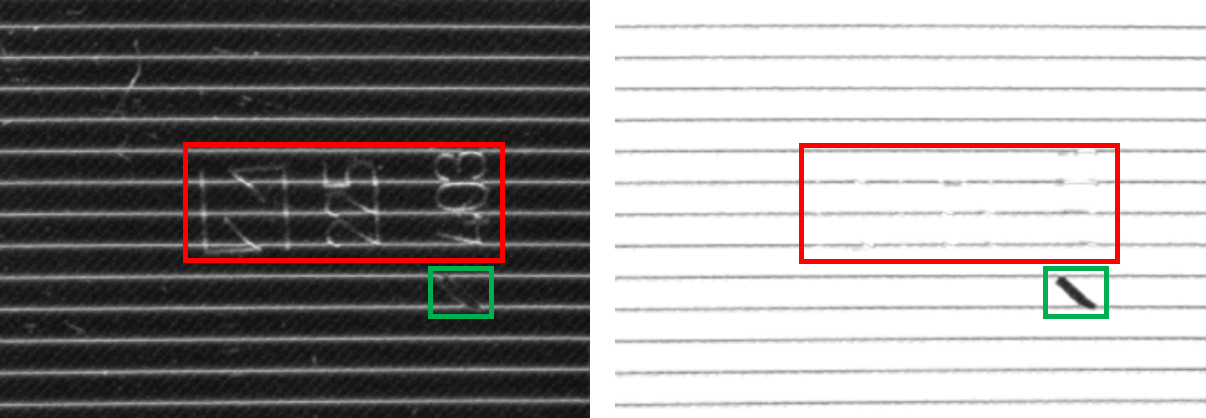
\includegraphics[width=\textwidth]{03_sichtpruefungDurchLichtstreuung/einsatzVonMehrerenStreifenmustern/figures/minAndMaxLink}
	\caption[Verknüpfte Bilder über Minimierung und Maximierung]{Verknüpfte Bilder, um Defekte von \textit{Fall 1} (rot umrahmt) und Defekte von \textit{Fall 2} (grün umrahmt) isoliert voneinander zu betrachten. Links über Minimierung und rechts über Maximierung verknüpft. Die verknüpften Quellbilder sind in Abbildung \ref{img:imageToLink} einzusehen.}
	\label{img:minAndMaxLink}
\end{figure}

\noindent
In den Bildern aus Abbildung \ref{img:minAndMaxLink} sind noch horizontale Streifen zu erkennen.
Diese sind keine Defekte, sondern entstehen aus Überlappungen der Streifenmuster in den Kamerabildern.
Auf diese \glqq Fehler\grqq ~und Möglichkeiten zur Beseitigung dieser wird im nächsten Abschnitt \ref{sec:optimierungen} ~eingegangen.

\p
Als Nächstes sollen beide Fälle in einem Gesamtbild kenntlich gemacht werden.
Hierfür macht man sich die Gemeinsamkeiten von \textit{Fall 1} und \textit{Fall 2} zunutze.
Man kann feststellen, dass die Helligkeit der Defekte in beiden Kamerabildern trotz Veränderung der Muster ungefähr gleich bleibt.
Verknüpft man die beiden Bilder durch die punktweise betragsmäßige Differenz, werden Defekte aus den beiden Fällen dunkel.
Die restliche, normal-spiegelnde Oberfläche wird hell, da jeder sonstige Bildpunkt in einem Muster dunkel und im anderen Muster hell erscheinen sollte, also eine hohe Differenz ergibt.
Die Ausnahme bilden dabei auch hier die Überlappungen von Streifen (siehe Abbildung \ref{img:diffImage}).

\begin{figure}[H]
	\centering
	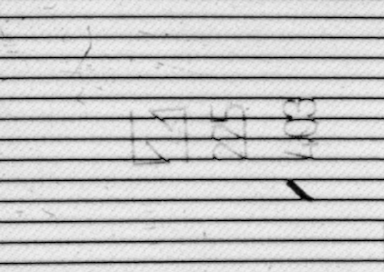
\includegraphics[width=0.5\textwidth]{03_sichtpruefungDurchLichtstreuung/einsatzVonMehrerenStreifenmustern/figures/diffImage}
	\caption[Verknüpfte Bilder über Differenz]{Über betragsmäßige Differenz verknüpfte Bilder.}
	\label{img:diffImage}
\end{figure}